\documentclass[a4paper,12pt]{report}

\usepackage[utf8]{inputenc}
\usepackage[francais]{babel}
\usepackage{fullpage,verbatim}
\usepackage{graphicx,ocamldoc}


\title{
  \textbf{Simulation du jeu de la vie avec l'algorithme Hashlife}
  \\ - \\
  Rapport de TER}
\author{Pierrick COUDERC et David MAISON
\\ - \\
Supervisé par Jean-Christophe FILLIÂTRE}

\begin{document}

\maketitle
\tableofcontents





\chapter{Introduction}\label{chap:intro}



\section{Contexte de travail}

Ce TER a été réalisé au LRI au sein de l'équipe TOCCATA, sous la direction de
Jean-Christophe FILLIÂTRE.

\section{Le jeu de la vie}
Le jeu de la vie, contrairement à son nom, n'est pas vraiment un jeu,
mais plutôt un automate cellulaire, inventé par John Conway en 1970.

Ce jeu se déroule sur une grille de dimension 2 de taille infinie qui évolue au
cours du temps.  Chaque cellule de la grille ne peut avoir que deux états :
vivante ou morte, et chaque cellule a donc un total de 8 cellules voisines.

Pour calculer l'état d'une cellule à l'itération suivante du jeu de la
vie, on applique les règles suivantes :
\begin{itemize}
\item Une cellule morte ne peut devenir vivante que s'il y a
  exactement 3 cellules voisines vivantes
\item Une cellule vivante ne peut le rester que s'il y a 2 ou 3
  cellules voisines vivantes, sinon elle meurt.
\end{itemize}
Donc pour calculer l'état d'une grille après un pas de temps, il faut
appliquer ces règles pour chaque cellule de la grille.



\section{L'algorithme Hashlife}\label{section:hashlife}

L'algorithme Hashlife a été proposé par Bill Gosper, un mathématicien et
informaticien américain en 1984, dans son l'article ``Exploiting regularities in
large cellular spaces''. Le principe de cet algorithme est de simuler des
automates cellulaires de taille gigantesque mais de manière efficace et
relativement rapide. Bien qu'il soit appliqué ici aux règles de Conway,
l'algorithme est applicable pour n'importe quel modèle cellulaire.

Le principe proposé par Gosper est d'exploiter la redondance des
configurations, et ainsi ne pas recalculer le résultat d'une partie de
l'automate qui aurait déjà été vue. De plus, l'algorithme permet de
calculer ce résultat dans un temps de \texttt{n-2} pas de temps, et
permet alors d'avancer très vite dans le temps pour une configuration
donnée. Un très bon exemple de l'intérêt de cet algorithme est une
configuration, un automate cyclique affichant le message
``Golly''. Celui-ci affichant un message en boucle, l'utilisation de
cette redondance pour le calcul est alors pertinente.

\begin{center}
  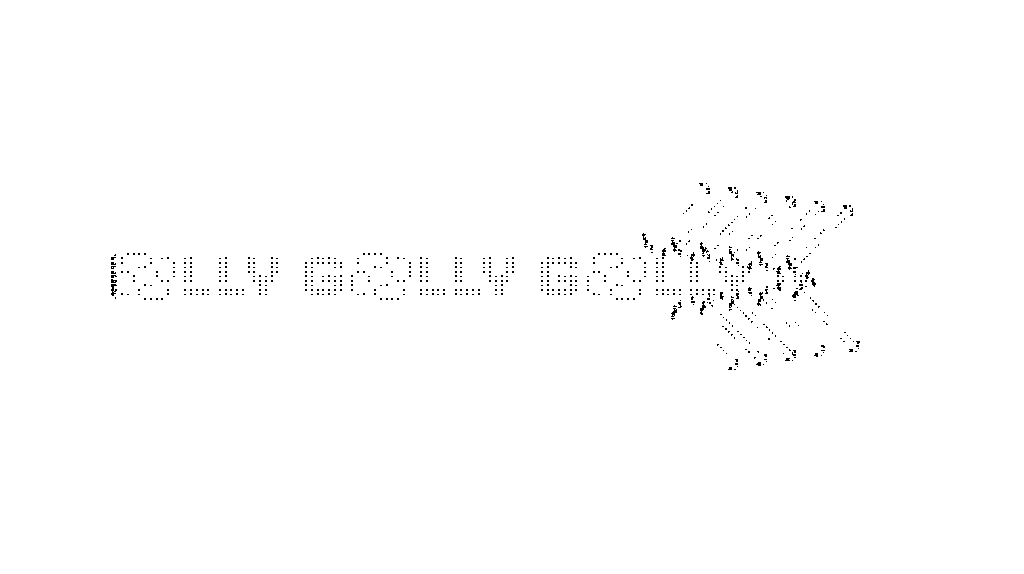
\includegraphics[scale=0.5]{screenshot_ticker.png}

  \textit{Le \texttt{ticker} qui imprime ``Golly''}
\end{center}

Le principe en lui même est le suivant :

Notre élément de base est appelé macro-cellule, c'est-à-dire une cellule de
2\textsuperscript{n} par 2\textsuperscript{n} cellules ``simples'' (ie. morte ou
vivante selon les règles de Conway). Cette même macro-cellule est elle-même
divisée en 4 macro-cellules de taille n-1 située dans chaque coin. Cette
structure est bien évidemment récursive jusqu'à obtenir une cellule de taille 0,
soit 2\textsuperscript{0} par 2\textsuperscript{0}, autrement dit une cellule
simple.

\medskip

Voici par exemple une macro-cellule contenant la configuration du
\texttt{glider} et sa représentation mémoire.

\begin{center}
    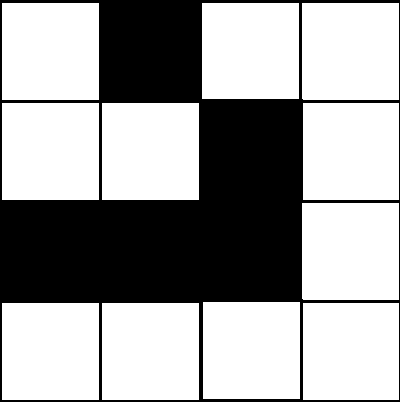
\includegraphics[scale=0.2]{glider_mc.png}

    \textit{Une macro-cellule de taille 2 représentant un ``glider''}

    \medskip

    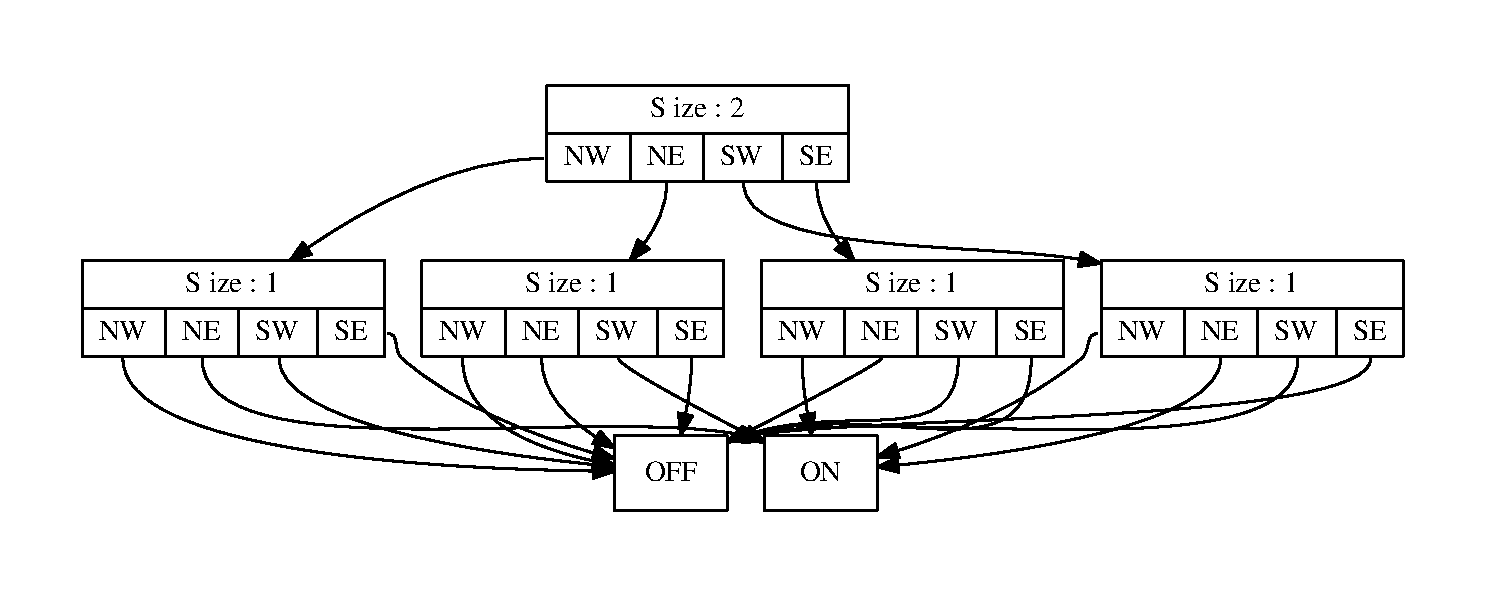
\includegraphics[scale=0.7]{glider.pdf}

    \textit{Sa représentation en mémoire}
\end{center}
\medskip

De plus, afin d'exploiter la redondance, ces macro-cellules sont uniques en
mémoire, c'est-à-dire que celles-ci sont hash-consées (voir plus loin). De cette
manière, une macro-cellule de taille n contenant deux macro-cellules filles
identiques aura simplement deux pointeurs vers la même macro-cellule. Une
macro-cellule peut être intuitivement vue comme un graphe orienté acyclique.

\medskip

\begin{center}
    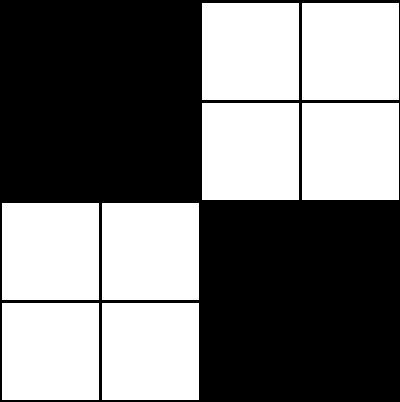
\includegraphics[scale=0.2]{redudancy_ex.png}

    \textit{Une macro-cellule de taille 2 avec redondance}

    \medskip

    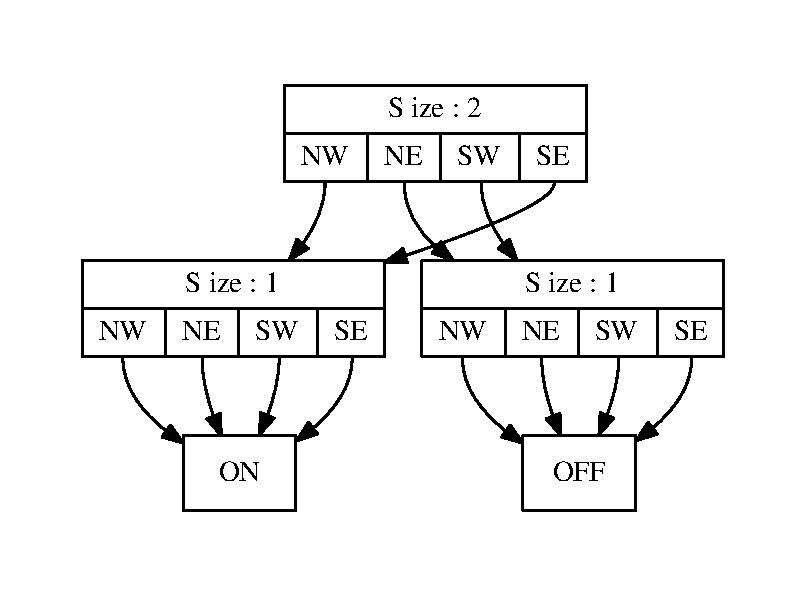
\includegraphics{redudancy.pdf}

    \textit{Sa représentation en mémoire}
\end{center}
\medskip

De cette manière, supposons une macro-cellule entièrement vide de taille 2, ses
4 coins pointeront donc vers la même macro-cellule de taille 1, qui elle-même
pointera vers le cas primaire ``OFF'', c'est-à-dire une cellule morte.

\medskip
\begin{center}
    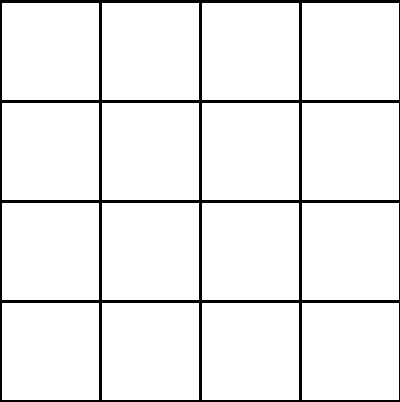
\includegraphics[scale=0.2]{emptycell.png}

    \textit{Une macro-cellule vide de taille 2}

    \medskip

    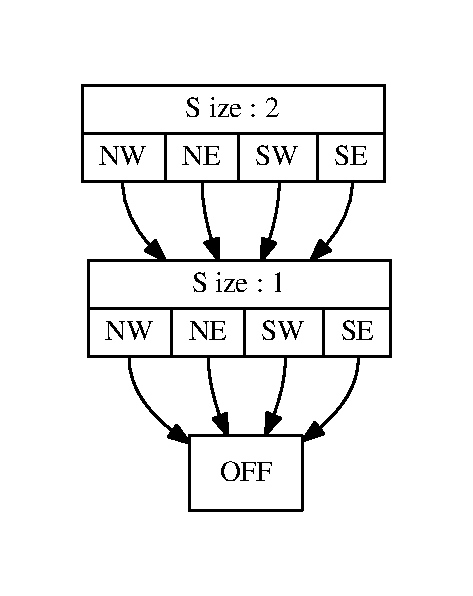
\includegraphics{empty2.pdf}

    \textit{Sa représentation en mémoire}
\end{center}

\medskip

Au final, une macro-cellule n'est donc composée que de 4 pointeurs, chacun pour
l'un des coins, ainsi que d'une information sur sa taille.


\subsection*{Résultat}


Celui-ci est le résultat de la macro-cellule donnée après
\texttt{n-2} pas de temps, mais pour le centre de celle-ci, soit une
macro-cellule de taille n-1. On a la certitude de pouvoir calculer le
centre du résultat dans tant de pas de temps, car celui-ci ne sera pas
affecté par la valeur de la \textit{couronne} qui l'entoure (i.e. la
macro-cellule à laquelle on aurait enlevé le centre). Pour cela, il
devient nécessaire de décomposer le calcul en 13 sous-parties, dont le
calcul du résultat sera ensuite appelé de manière récursive, jusqu'au
cas de base qui est lui calculé directement via les règles du Jeu de
la vie. 

La décomposition du calcul consistera alors en les étapes
suivantes, pour obtenir une macro-cellule intermédiaire qui permettra
d'obtenir le résultat :


La première partie sera de calculer les coins de la macro-cellule
  intermédiaire.

\medskip
\begin{center}
  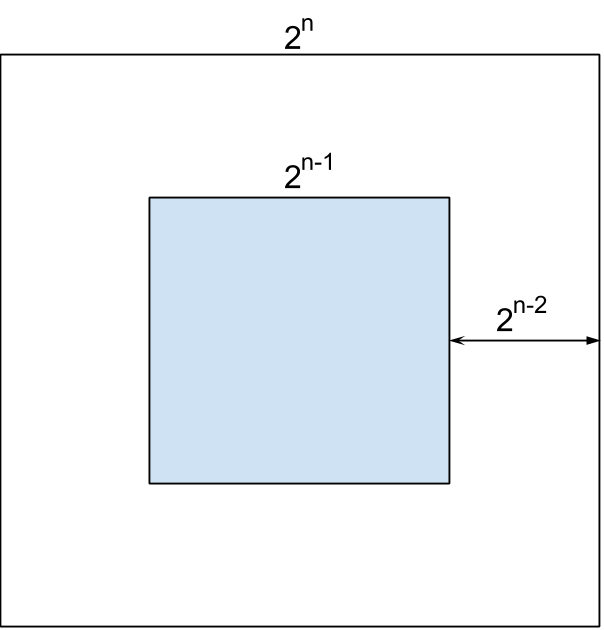
\includegraphics{result.mps}
\end{center}
\medskip

La deuxième étape est de recomposer des macro-cellules pour ainsi obtenir
  la cellule du centre ainsi que celle au nord, au sud, à l'est et à l'ouest. 

\medskip
\begin{center}
  \includegraphics{result2.mps}
\end{center}
\medskip

Enfin, les 9 sous-parties devront être ré-assemblées puis leur résultat
  calculé pour ensuite composer la macro-cellule résultat.

\medskip 
\begin{center}
  \includegraphics{result3.mps}
\end{center}
\medskip

Le résultat est encore une fois mémoïsé, ce qui permet
d'accélérer de manière importante le calcul des automates présentant
une grande redondance. Celle-ci sera faite à l'aide
d'un pointeur directement dans la structure de la macro-cellule, qui
pointera directement vers son résultat. De cette manière, si ce
résultat n'existe pas, ce pointeur ne pointera vers rien et il
conviendra donc de le calculer, sinon seulement de le renvoyer.





\subsection*{Mémoïsation et hash-consing}\label{section:hashconsig}

La mémoïsation est une technique de qui a pour but ne pas refaire une
opération qui a déjà été faite auparavant. Une telle opération peut être
de n'importe quel type, comme des opérations arithmétiques ou comme
dans notre cas, par exemple, la construction de macro-cellules.

Le principe est simple : on initialise d'abord une table de hachage
vide. Lorsqu'on lance l'opération, on vérifie dans la table de
hachage si elle n'a pas déjà été faite, si oui, alors on renvoie le
résultat qui lui était associé dans la table de hachage. Sinon on
procède au calcul, et on enregistre ce calcul dans la table de hachage
en lui associant son résultat, avant de renvoyer le résultat de
l'opération.

Le hash-consing est un cas particulier de la mémoïsation, où l'opération
considérée est une opération d'allocation mémoire.

Le hash-consing a pour conséquence dans l'immédiat de gagner en mémoire au
profit d'un peu de temps de calcul, ce qui est normal car pour ne pas
enregistrer ce qui a déjà été fait, il faut vérifier qu'il n'a pas déjà été
construit, et le construire le cas échéant.  Cependant, lorsqu'on va effectuer
des actions ou des calculs sur les données hash-consées, on gagnera aussi en
temps en mémoïsant le résultat du calcul. Par conséquent, plus il y a
d'opérations redondantes, plus le hash-consing sera efficace.  Ce qui est
souvent notre cas dans le jeu de la vie pour des macro-cellules de petites
tailles ou bien pour des macro-cellules vides qui sont très présentes.












\chapter{Implémentation}\label{chap:implement}

Par la suite, notre implémentation est faite en OCaml.

\section{Le module Mcell}\label{section:mcell}

\subsection*{Le type mcell}

Pour modéliser les macro-cellules, il a été nécessaire de créer un type
particulier : 
\begin{verbatim}
type t = { 
  id : int; 
  size : int; 
  nw : t; 
  ne : t; 
  sw : t; 
  se : t; 
  mutable result : t 
}
\end{verbatim}

Ainsi les quatre champs \textit{nw}, \textit{ne}, \textit{sw} et \textit{se}
représentent respectivement les macro-cellules filles situées au Nord-ouest,
Nord-est, Sud-ouest et Sud-est. Il s'agit donc d'un type récursif. La
macro-cellule contient également un pointeur vers son résultat (s'il a déjà été
calculé) et enfin, un champ id pour permettre le hachage des
macro-cellules. La taille de la macro-cellule est également conservée.

Dans le cas où le résultat n'a pas été calculé, le champ \texttt{result}
pointera vers une variable particulière nommée \texttt{null}, qui représente un
pointeur nul (de la même manière que dans d'autres langages, tels que C ou Java).

\medskip

%% Pour réaliser de la mémoïsation sur ce type précis, il était nécessaire de
%% trouver une fonction de hachage efficace, et de même pour une fonction
%% d'égalité. Grâce justement à cette mémoïsation, lors de la création d'un
%% élément, si celui-ci est déjà en mémoire on ne fera alors que pointer sur ce
%% dernier. De cette manière, il est possible d'utiliser l'égalité physique et non
%% l'égalité structurelle. Il est néanmoins impossible de comparer les champs id,
%% car ce champ, lors de la création d'une macro-cellule, est déterminé
%% arbitrairement avant de savoir si une macro-cellule construite de la même
%% manière existe déjà. En revanche, la fonction de hachage utilisera ce champ.

La mémoïsation est réalisée seulement à la création de la
macro-cellule. Cette fonction de création est du type suivant :
\begin{verbatim}
val create : nw:t -> ne:t -> sw:t -> se:t -> t
\end{verbatim}

Une nouvelle macro-cellule sera d'abord créée avec un id arbitraire, et on fera
ensuite une recherche dans la table de hachage dans le but de trouver s'il
existe déjà un élément construit avec ces mêmes macro-cellules filles (et bien
évidemment dans le même ordre). Si celle-ci n'existe pas, on l'ajoutera alors
dans la table, dans le cas contraire on renverra l'existante. On garanti ainsi
l'unicité des macro-cellules. La possibilité de comparer les macro-cellules
filles est garantie justement par ce hash-consing, celles-ci ayant été créées
auparavant. 

Bien sûr, il est impossible de composer une macro-cellule avec des
macro-cellules filles qui seraient de tailles différentes, puisqu'il faut
garantir la propriété qu'une cellule sera toujours de taille 
2\textsuperscript{n}.

\medskip

Finalement, le module suivant permet au foncteur de Hashtbl d'effectuer la
mémoïsation :
\begin{verbatim}
module T = struct
  type t = mcell
  let equal m1 m2 =
    m1.nw == m2.nw && m1.ne == m2.ne && m1.sw == m2.sw && m1.se == m2.se
      
  let hash m = abs (19 * (19 * (19 * m.nw.id + m.ne.id) + m.sw.id) + m.se.id)
end
\end{verbatim}

Il est important de préciser que le type \texttt{t} est privé. De cette manière,
il est nécessaire d'utiliser la fonction \texttt{create} pour créer une
macro-cellule et de cette manière garantir le hash-consing et donc l'unicité en
mémoire des constructions. 

Le hash-consing permet de garantir le résultat suivant pour deux macro-cellules
\texttt{x} et \texttt{y} quelconques :

\begin{equation}
   x = y \Leftrightarrow x == y \Leftrightarrow x.id = y.id
\end{equation}

\medskip



\subsection*{Calcul du résultat}

L'idée générale de l'algorithme est bien évidemment de calculer le résultat
d'une macro-cellule dans un temps de 2\textsuperscript{n-2} pas de temps, où
\textit{n} est la taille de la macro-cellule elle-même. Pour cela, il convient
de réaliser un assemblage comme vu dans le chapitre
\ref{section:hashlife}. Ainsi donc, le calcul met lui aussi en \oe uvre le
principe de la mémoïsation grâce au champ mutable result.

Si celui-ci est égal à null, le calcul du résultat doit donc être effectué, dans
le cas contraire, il suffit de renvoyer la macro-cellule pointée par le
champ. Si calcul il doit y avoir, alors le calcul est effectué récursivement
jusqu'à arriver à un \textit{result} déjà calculé ou dans le cas contraire, dès
que l'algorithme atteint une cellule de taille 3 de calculer
directement le résultat à l'aide des règles du jeu de la vie.

De cette manière, et puisque les macro-cellules sont uniques en mémoire, lorsque
l'algorithme calcule un résultat, s'il voit une nouvelle fois la même
macro-cellule il n'aura pas besoin de recalculer le résultat.

\subsection*{La fonction future}

Grâce au résultat nous pouvons calculer l'état d'une macro-cellule
dans pour un pas de temps k de 2\textsuperscript{n-2} avec n la taille
de la macro-cellule. Cependant il se peut qu'on veuille par moment
avancer d'un pas de temps quelconque.
Dans le cas où cette puissance de 2 est supérieure à n-2, il suffit
d'étendre la macro-cellule avec du vide pour que sa taille
corresponde, mais dans le cas où la puissance de 2 est inférieure, il
va falloir procéder autrement.
Pour cela, nous allons reprendre le principe de découpage des
macro-cellules utilisé pour le résultat.

Le principe est le suivant : on va procéder récursivement en calculant
le ``futur'' des 4 macro-cellules situées au centre comme lors du calcul du
résultat. Et dès qu'on atteint une macro-cellule fille qui a une taille
qui correspond à notre pas de temps, alors on va calculer et renvoyer
le résultat de cette macro-cellule.

\medskip

Donc à la fin nous aurons une macro-cellule qui sera un assemblage des
résultats des macro-cellules filles de taille k+2.

Pour aller plus loin : si on veut avancer d'un pas de temps qui n'est pas à
l'origine une puissance de 2, il suffit de décomposer ce pas de temps en une
somme de puissance de 2 et appliquer notre fonction \texttt{future} avec chaque
terme de cette somme en reprenant à chaque fois la macro-cellule qui vient
d'être modifiée.

\subsection*{Des extensions du module}

En plus des fonctions propres au jeu de la vie, pour étendre notre
module Mcell, nous avons ajouté des fonctions qui permettent
de modifier ou de transformer une macro-cellule.

Parmi ces fonctions nous retrouvons :
\begin{itemize}
\item \texttt{union} : fabrique une macro-cellule qui est l'union de deux
  macro-cellules (qui résulte de l'union de chaque cellules atomique).
\item \texttt{inter} : fabrique une macro-cellule qui représente l'intersection
  de deux macro-cellules.
\item \texttt{diff} : fabrique une macro-cellule qui représente la différence
  entre deux macro-cellules.
\item \texttt{mirror} : renvoie la même macro-cellule en appliquant une
  symétrie axiale verticale.
\item \texttt{rotate90/180/270} : renvoie la même macro-cellule en appliquant
  une rotation de 90, 180 ou 270 degrés dans le sens trigonométrique.
\item \texttt{extend-left/right} : ajoute un espace blanc à gauche (droite) de
  la macro-cellule d'origine.
\end{itemize}

Toutes ces fonctions, mises à part les ``extend'', utilisent la
mémoïsation afin d'exploiter au maximum le hash-consing effectué et
gagner en temps de calcul et en mémoire. Cependant, chaque fonction a
sa propre table de hachage, ce qui peut poser un problème en terme de
mémoire. En effet, et c'est un des problèmes du hash-consing, on peut avoir de
certitude quant à l'utilité par la suite d'avoir hash-consé ces opérations et il
peut alors être plus intéressant de \textit{vider} ces tables à la fin de
l'opération sur la macro-cellule complète. Mais évidemment, cela peut être un
problème dans le cas où il faudrait alors refaire cette opération par la suite
car il n'y aurait plus de hash-consing.
%% , il y en a donc un certain nombre, et si
%% elles ne sont pas vidées, on risque de prendre beaucoup trop de
%% mémoire, surtout qu'on utilise peu souvent ces fonctions. Mais si on
%% les vide à chaque application de ces fonctions, si on fait par exemple
%% cinq fois une union, il se peut qu'on perde en efficacité.

\medskip

Par conséquent, nous avons adopté la solution suivante : les tables de
hachage sont globales et nous mettons à disposition de l'utilisateur
une fonction pour vider les tables quand il le souhaite, pour ainsi
optimiser l'utilisation et la mémoire que prenne ces tables. Nous
pouvons y voir un intérêt avec notre langage Mcop qui sera présenté
plus loin.


\section{Les modules de parsing de fichiers}\label{section:parsing}

Il existe deux formats de fichier de descriptions pour le jeu de la vie,
l'Extended RLE, un descripteur simple et standard dérivé d'un format de
compression, et le MC, spécifiquement créé pour utiliser les propriétés de
la représentation d'une macro-cellule selon Hashlife.

\subsection{Le format RLE}

Le format Extended RLE (pour ``Run-Length Encoding'') est à la base un format de
compression mis au point pour l'impression de documents en noir et blanc, dont
le principe était de concaténer les pixels voisins de même couleur sur une même
ligne. Celui-ci a ensuite été adapté pour le jeu de la vie avec quelques ajouts
(d'où la mention ``Extended''), tout particulièrement un en-tête permettant la
description de l'automate cellulaire utilisé et la taille de la grille adaptée.

Le fichier est ainsi divisé en deux parties distinctes : l'en-tête et la
description. L'en-tête est construit de la manière suivante :
\begin{verbatim}
x = 3, y = 3, rule = B3/S23
\end{verbatim}

Trivialement, x et y définissent la taille de la grille du jeu de la
vie qui sera nécessaire pour afficher l'ensemble des cellules
décrites. L'argument rule cependant est plus intéressant : il permet
de définir les règles utilisées par l'automate cellulaire. Ainsi, le
RLE n'est pas adapté seulement aux règles de Conway mais
également à des configurations plus exotiques. L'argument passé à rule
est divisé en deux parties : B et S. La lettre et le (ou les)
chiffre(s) qui suivent indiquent au programme le nombre exact de
cellules voisines nécessaire à une cellule morte (\textbf{B}) pour revivre ou une
cellule vivante (\textbf{S}) pour rester en vie. Ainsi, B3 signifie
qu'une cellule morte aura besoin de 3 cellules vivantes pour revenir à
la vie, et S23 qu'une vivante ne pourra le rester que si
elle en a 2 ou 3 autres encore en vie parmi ses 8 voisins.

Pour la description, prenons par exemple celle du glider :
\begin{verbatim}
bo$2bo$3o!
\end{verbatim}
La description est composée des éléments suivants :
\begin{itemize}
\item \textbf{b} pour une cellule morte
\item \textbf{o} pour une cellule vivante
\item \textbf{\$} pour un retour à la ligne
\item \textbf{!} (optionnel) qui indique la fin de la description
\end{itemize}

Chacun de ces caractères (excepté le \textbf{!}) peuvent être précédés
d'un nombre, indiquant alors le nombre de fois où cet élément est
répété sur la ligne actuelle. Par exemple, 3o signifiera que 3
cellules vivantes sont situées côte-à-côte sur la même ligne, tandis
que 3\$ indiquera qu'il faut sauter trois lignes pour continuer la
description. Il n'est pas nécessaire de compléter une ligne avec le
nombre exact de cellules qu'elle contient : une ligne non terminée
sera automatiquement remplie jusqu'à la fin avec des cellules
mortes. C'est ce qui d'ailleurs justifie de pouvoir sauter plusieurs
lignes à la fois.

Enfin, bien que cela n'ait qu'un intérêt pratique et non algorithmique, le
format supporte les commentaires lignes par lignes (précédés d'un \textbf{\#}) 
avant le header et avant la partie de description.

\medskip

L'algorithme décrivant cellule par cellule le tableau du jeu de la vie, il a
donc été nécessaire de trouver un moyen de créer une macro-cellule. La première
étape a donc été de créer une matrice de booléens qui serait ensuite convertie
en macro-cellule, mais cette solution n'était pas satisfaisante : en effet, on
peut imaginer par exemple que le RLE décrirait une macro-cellule immense mais
avec seulement trois cellules vivantes. La matrice serait gigantesque pour très
peu, et l'ouverture d'un fichier prendrait alors une place énorme en mémoire
(même pour un temps très court).

Nous avons donc créé une fonction \texttt{set} par la suite qui, prenant une
macro-cellule vide et des coordonnées x et y, allume (ou éteint) la
cellule à l'emplacement donné. On réalise alors autant d'opérations \texttt{set}
qu'il y a de cellules allumées.

Au final, le prototype de \texttt{set} est le suivant :
\begin{verbatim}
val set : t -> int -> int -> bool -> t
\end{verbatim}


\subsection{Le format MC}
Le format est un format de fichier imaginé pour exploiter la réprésentation des
macro-cellules sous forme de quadtrees. Il s'agit d'ailleurs de l'acronyme pour
``Macro-Cells''.  Prenons l'exemple simple encore fois d'un glider. Le fichier
serait alors de cette forme :

\begin{verbatim}
#made with hashlife-ocaml
$$..*$...*$.***$$$$
4 1 0 0 0
\end{verbatim}

Comme pour le RLE, les commentaires sont admis, et certains fichiers possèdent
également un en-tête qui est rajouté automatiquement par le programme ayant créé
le fichier. Néanmoins, ces derniers n'ont aucune utilité pratique mais seulement
informatives.

Le fichier est essentiellement constitué de la description de la macro-cellule
qui doit être créée, et pour cela le format utilise deux descriptions
différentes :

Une première, qui est de ce type :
\begin{verbatim}
$$..*$...*$.***$$$$
\end{verbatim}
Il s'agit de la description d'une macro-cellule de taille 3 (8 par 8 cellules),
description ligne par ligne à la manière d'un RLE. Ainsi, un \textbf{.}
symbolise une cellule morte, un \textbf{*} une cellule vivante et \textbf{\$}
une fin de ligne. C'est également la brique de base pour la construction de
macro-cellules : de cette manière, la macro-cellule créée par le MC ne pourra
jamais avoir une taille inférieure à 8 par 8 cellules.

Le second type est différent : 
\begin{verbatim}
4 1 0 0 0
\end{verbatim}
Cette ligne est également une macro-cellule, mais qui utilise des éléments déjà
créés auparavant dans le fichier. Ainsi, le premier chiffre est la taille de la
macro-cellule. Les 4 suivants sont les numéros dans l'ordre de création des
macro-cellules déjà créées, dans l'ordre Nord-ouest, Nord-est, Sud-ouest,
Sud-est. La numérotation commençant à 1, le zéro indique une cellule totalement
vide de taille n-1 à celle qui est en cours de création.

Le résultat final est la dernière macro-cellule créée.

\medskip

On peut ainsi voir que le format ainsi créé utilise exactement la structure de
la macro-cellule avec partage. D'ailleurs, notre bibliothèque permet l'export de
macro-cellules vers ce format qui garanti que chaque ligne du fichier MC est
unique.

\section{Le module graphique}

\subsubsection*{Un problème d'affichage}

Nous voulons afficher à l'écran notre macro-cellule, qui comme vu en
2.1 est en fait un arbre. Donc on va devoir parcourir cet arbre de
manière récursive jusqu'aux feuilles pour savoir si on va dessiner un
pixel noir ou rien. Cependant ce n'est pas si simple.

\medskip

Tout d'abord supposons que nous voulons afficher toute la
macro-cellule mère dans tout l'écran, il va falloir donner des
coordonnées (x,y) de l'écran pour savoir lors d'un parcours récursif
où on en est dans la macro-cellule mère, sinon au niveau de la feuille
on va vouloir dessiner un pixel sans savoir où on doit le faire.

On prend la convention suivante : la feuille tout en haut à gauche
aura pour coordonnée (0,0) et celle tout en bas à droite
(2\textsuperscript{n-1}, 2\textsuperscript{n-1}) avec n la dimension
de la macro-cellule mère. On a vu que chaque macro-cellule de taille n
est constituée de 4 macro-cellules de taille n-1, donc la feuille tout
en haut à gauche de la macro-cellule fille nord-est aura pour
coordonnée (2\textsuperscript{n-1}/2, 0), et ainsi de suite pour les
autres macro-cellules filles.

De cette façon, avec notre parcours de l'arbre tout en passant les
coordonnées de là où on se situe dans notre écran, on va pouvoir
dessiner des pixels qui correspond réellement à notre configuration du
jeu de la vie.

Il reste juste à choisir une variable de mise à l'échelle pour dire
qu'une cellule n'est pas un pixel mais un rectangle afin de remplir
tout l'écran avec notre macro-cellule mère.

\medskip

Cependant, on se rend vite compte qu'il est parfois, voire souvent,
inutile de parcourir l'arbre jusqu'aux feuilles dans les cas où notre
macro-cellule de taille n est vide car dans tous les cas, on ne
dessinera rien. Surtout que les cellules vides sont très présentes
dans nos configurations. Et de même pour une macro-cellule pleine, il
suffit de dessiner qu'un seul grand rectangle et non pas plein de
petit rectangle qui seront au final côte à côte.  Avec cette petite
optimisation, on va un temps considérable lors de l'affichage d'une
macro-cellule.

\medskip

De plus, il sera plus aisé pour certaine grosse configuration du jeu
de la vie de pouvoir se déplacer et zoomer dans cette macro-cellule
mère, et bien sûr on ne veut pas parcourir les parties de l'arbre qui
ne seront pas affichées sous peine d'avoir des performances très
médiocres.

Donc autrement dit, on va vouloir dessiner une partie de la
macro-cellule, pour faire simple : afficher une sélection
rectangulaire de cette dernière.

On va alors procéder à un parcours récursif sur les parties de l'arbre
concernée tout en découpant notre sélection rectangulaire : donc à
chaque appel récursif on aura à notre disposition une macro-cellule et
une sélection rectangulaire.

La découpe est assez simple et on différencie principalement 3 cas :
\begin{itemize}
\item Soit la sélection est totalement incluse dans une des
  macro-cellules filles, dans ce cas on ré-appelle avec la même
  sélection dans la macro-cellule en question sauf si cette
  macro-cellule est vide (dans ce cas on ne fait plus rien) ou pleine
  (et on dessine un rectangle noir à l'écran).
\item Soit la sélection chevauche deux macro-cellules filles, alors on
  découpe la sélection en 2 et on ré-appelle sur les deux
  macro-cellules filles avec leur sélection correspondantes.
\item Soit la sélection chevauche les 4 macro-cellules, et le
  traitement est le même que pour 2 mais étendu sur les 4
  macro-cellules filles.
\end{itemize}
Cette découpe nous permet ainsi d'avoir le bon parcours de l'arbre
voulu puisque récursivement on ira jamais dans des branches inutiles,
et on arrivera forcement au cas 1 où la sélection couvre toute la
macro-cellule (au pire c'est une cellule).

Cependant, vu qu'on ne veut pas forcement afficher toute la
macro-cellule quand on fait un appel récursif, comment savoir laquelle
des macro-cellules filles on va devoir afficher ? Pour rappel nous
n'avons que les coordonnées (x,y) qui correspondent à la position dans
l'écran.

\medskip

Prenons l'exemple suivant :


\begin{center}
  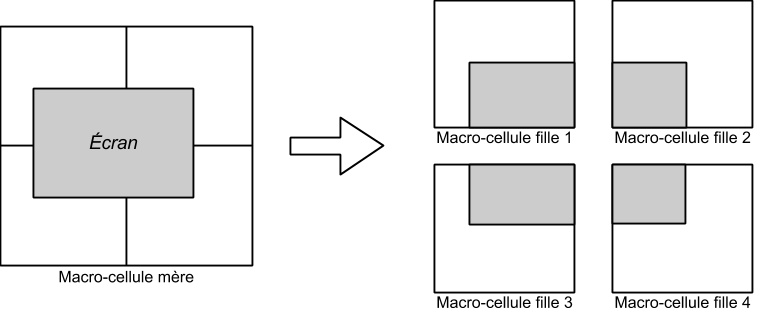
\includegraphics[scale=0.5]{decoupage_graphique.png}
\end{center}


Pour la macro-cellule fille 2, nous connaissons les coordonnées (x,y)
pour dessiner à l'écran mais on ne veut pas afficher toute la
macro-cellule, que la partie de la sélection. Et donc pour savoir où
on doit s'arrêter, il faut connaître la taille de la sélection
(largeur w et hauteur h).
Pour la macro-cellule fille 3, les coordonnées (x,y) sont (0,0) mais
on ne veut pas afficher les cellules situées en bas à gauche. Il va
donc falloir d'autres coordonnées (i,j) qui correspondent aux
coordonnées dans la macro-cellule à partir desquelles on va afficher
les cellules à l'écran.

\medskip

Donc il nous faut 3 types de données :
\begin{itemize}
\item Les coordonnées (x,y) de l'écran pour savoir où on affiche
\item Les coordonnées (i,j) de la macro-cellule pour ne pas parcourir
  les cellules situées avant les coordonnées de la sélection
\item La taille (w,h) de la sélection pour ne pas parcourir les
  cellules situées après les coordonnées de la sélection
\end{itemize}

Il reste donc juste à calculer les coordonnées en (x,y) et les bonnes
découpes à faire pour lancer le procédé récursif, et nous avons notre
affichage générique optimisé. Pour se déplacer dans la macro-cellule
mère, il suffira de déplacer la sélection, et pour zoomer, de réduire
la taille de cette dernière, le tout en ignorant les
sélections/parties de la sélection qui sortent de la macro-cellule (et
donc seront forcement vides).

\subsubsection{Implémentation avec le module Graphics}

Afin d'implémenter l'algorithme de découpage simplement, nous avons
tout d'abord utiliser la librairie standard Graphics de OCaml.
Cette application se contente donc d'afficher une macro-cellule et de
se déplacer/zoomer dedans à l'aide de touches du clavier.

On a aussi ajouter d'autres fonctionnalités de bases liées aux
macro-cellules comme jouer une itération dans n pas de temps (pouvant
être modifié par l'utilisateur), ainsi qu'une animation.

\subsubsection{Implémentation avec Gtk-Cairo}

Une fois le projet bien avancé, nous ne pouvions nous limiter à Graphics et nous
avions cherché à créer un logiciel plus professionnel avec une vraie interface
graphique, et notamment des interactions avec la souris.

Nous avons donc choisi d'utiliser la librairie Gtk qui nous permet de
créer une interface avec des widgets très facilement.
Cependant le widget de dessin de Gtk est assez primitif et nous avons
préféré nous tourner vers du dessin vectoriel. Cairo étant assez
utilisé pour ceci et déjà interfacé dans Gtk, nous l'avons
donc choisi.

Cette nouvelle application propose donc toutes les anciennes
fonctionnalités disponibles avec Graphics au clavier, mais aussi avec
des boutons. De plus on peut aussi manier la macro-cellule et se
déplacer à l'aide de la souris, et effectuer des zooms plus précis.

\begin{center}
  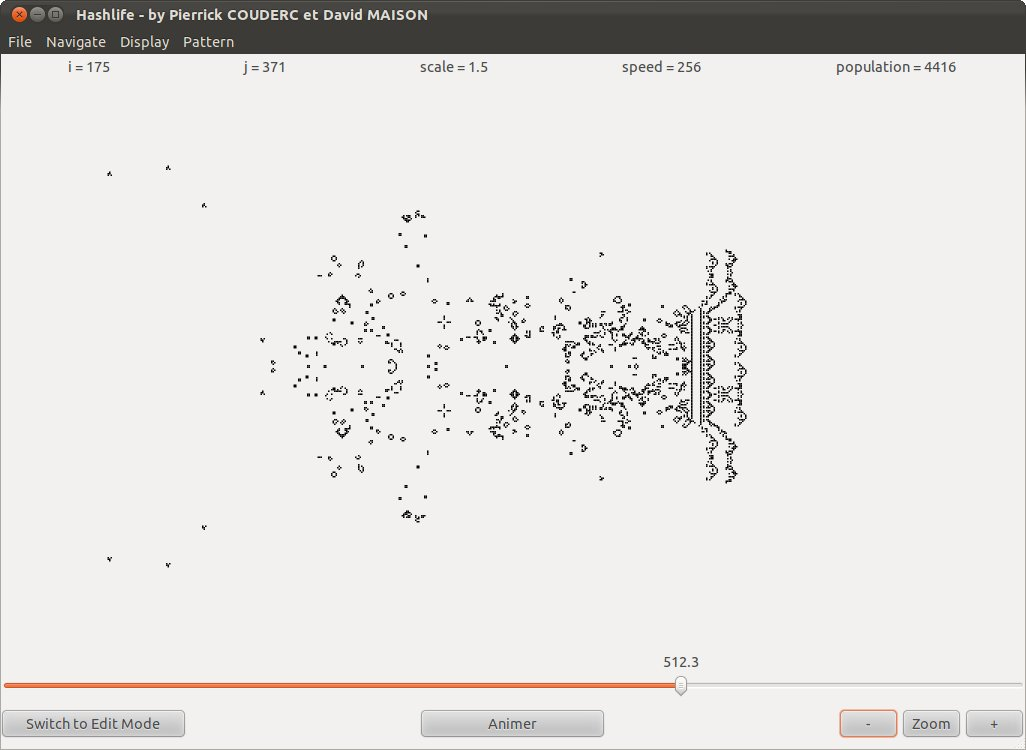
\includegraphics[scale=0.4]{screenshot.jpg}
\end{center}

\section{Le langage Mcop}

Après avoir écrit tout ce qui était nécessaire pour exécuter l'algorithme
Hashlife, nous avons eu l'idée d'écrire des opérations booléennes sur des
macro-cellules. En effet, celles-ci peuvent être vues comme des matrices de
booléens et il est donc facile de réaliser des unions ou des intersections par
exemple entre deux macro-cellules de même taille. Pour ensuite utiliser ces
extensions de manière efficace, nous avons écrit un langage très simple capable
de réaliser ces opérations. La syntaxe est très simple et inspirée largement de
celle d'OCaml, à base de let ... in, et donc l'opération finale est la
macro-cellule à afficher (ou à écrire dans un fichier).

Ce langage permet donc plusieurs types d'opérations, dont voici un exemple :
\begin{verbatim}
let a = readrle("files/glider.rle") in
let b = mirror(a) in
union(a, b)
\end{verbatim}

Ainsi nous pouvons implémenter les fonctions du module Mcell suivantes :
\begin{itemize}
\item Les opérations binaires d'union, intersection et différence (ou XOR)
\item Les opérations unaires : le miroir vertical, les rotations à 90, 180 et
  270 degrés
\item Les opérations d'extension de taille des macro-cellules, qui peuvent
  augmenter de 1 la taille de 1 des macro-cellules en rajoutant de la bordure,
  ou de l'espace blanc à gauche ou à droite
\item La lecture des fichiers RLE ou MC
\end{itemize}

Il est également possible de sauvegarder le résultat de ces opérations dans un
fichier RLE ou MC, de la manière suivante :
\begin{verbatim}
let a = readrle("files/glider.rle") in
let b = mirror(a) in
let c = union(a, b) in
outmc(c, "double_glider.mc")
\end{verbatim}

Dans ce cas précis, le résultat ne sera pas affiché dans le programme et
seulement la sauvegarde sera faite.

\medskip

Ces opérations utilisent les fonctions du module Mcell
qui utilisent les tables de hachage pour la mémoïsation. De plus la
principale utilisation de ce langage Mcop est de faire des opérations
sur les macro-cellules, puis l'afficher ou enregistrer la
macro-cellule résultat. Par conséquent, les calculs ne seront fait que
lors de l'exécution du langage, et on va pouvoir optimiser ainsi la
mémoïsation et la mémoire utilisée par les tables de hachage en les
vidant qu'une fois toutes les opérations effectuées. Ceci n'aurait pas
été possible et nettement moins optimisé si les tables n'était pas
globale et donc vidées à chaque opération, et de même, si on n'avait
pas fait de fonctions pour vider les tables, alors même après ces
opérations, les tables prendraient de la place en mémoire (parfois
beaucoup si les macro-cellules sont grosses) alors qu'on ne les
utiliseraient plus.

\medskip

On peut aussi signaler que si le module Mcell est enrichi par la
suite, il peut alors être facile d'enrichir aussi ce langage pour
réutiliser les fonctions du module.

Il aurait pu être aussi intéressant de pouvoir utiliser les fonctions
``create'' des macro-cellules, mais dans ce cas, il faudrait faire une
vérification de la taille des macro-cellules. Cependant cette
vérification ne peut être forcement statique au moment du parsing du
fichier Mcop, car si on utilise la lecture d'un fichier Rle, on ne
peut connaître la taille que lors de l'exécution. C'est néanmoins
possible de le faire et peut être l'objet d'une extension intéressante
du langage.


\chapter{Tests et performances}

Dans ce chapitre, nous allons mesurer les performances de notre
logiciel, aussi bien au niveau de la mémoire que du temps d'exécution.
Ces tests vont être effectués sans affichage graphique, autrement dit,
les résultats que nous allons vous présentés indiquent les
performances des opérations sur les macro-cellules elles-mêmes.

\section{Tests généraux sur des fichiers Rle/MC}

Comme premiers tests, nous allons prendre des fichiers Rle et MC de
tailles différentes.
Pour rappel, chaque macro-cellule sont représentées comme des
quadtrees en mémoire, donc nous allons vous présenter le nombre de
n\oe uds que contiennent ces arbres : ceci reflète donc l'état de la
mémoire.
De plus, nous calculons le temps de construction de la macro-cellule
depuis l'ouverture du fichier et pendant la conversion des données
dans notre type Mcell.
Et pour démontrer l'efficacité de l'algorithme Hashlife, nous
calculons aussi le temps que prend le calcul du résultat de la
macro-cellule.
Enfin, à titre indicatif, nous vous donnons aussi le nombre de
cellules vivantes dans chaque configuration du jeu de la vie.

\begin{center}
  \begin{tabular}{| c | c | c | c | c | c |}
    \hline
    nom du fichier & taille (2\textsuperscript{n}) & cellules vivantes
    & n\oe uds & temps de création &
    calcul du résultat \rule[-7pt]{0pt}{20pt} \tabularnewline
    \hline
    glider.rle & 1 & 5 & 7 & 0.001s & 0.000s \tabularnewline
    puffer.rle & 7 & 878 & 274 & 0.020s & 0.017s \tabularnewline
    broken-lines.mc & 8 & 1766 & 611 & 0.020s & 0.088s \tabularnewline
    turing.rle & 10 & 36549 & 9384 & 1.808s & 6.384s \tabularnewline
    ticker.rle & 11 & 5043 & 2072 & 0.162s & 1.158s \tabularnewline
    memory-loop.rle & 14 & 12947 & 4164 & 0.848s & 0.536s \tabularnewline
    hexadecimal.rle & 15 & 2104670 & 6912 & 90.128s & 11.463s \tabularnewline
    hexadecimal.mc & 15 & 2104670 & 6912 & 0.143s & 11.678s \tabularnewline
    \hline
  \end{tabular}
\end{center}

Avec ces résultats, nous pouvons constater d'une part l'efficacité
flagrante du format MC par rapport au format Rle sur les fichiers
``hexadecimal'' sur le temps de création de la macro-cellule.

Nous pouvons voir aussi que dans le cas du fichier turing.rle, la
configuration est assez chaotique et sans redondance, d'où le nombre
de n\oe uds assez grand et un temps de calcul plus grand (on rappelle
que le calcul du résultat donne l'état de la configuration dans n-2
pas de temps avec n la taille de la macro-cellule).

Dans tous les cas, nous observons quand même un temps de calcul de
résultat infiniment petit comparé à la taille des macro-cellule. Cela
va de soi qu'un tel calcul en force brute en appliquant naïvement les
règles du jeu de la vie est tout simplement impossible à une échelle
de 2\textsuperscript{11} pour le ticker par exemple. De même, en ce
qui concerne la représentation en mémoire de ces configurations, si
on l'avait fait naïvement avec une matrice de booléen, pour le ticker,
cela aurait pris une quantité colossale de mémoire, alors qu'avec
Hashlife il ne prend que 2072 n\oe uds de type Mcell en mémoire. 


\section{Tests sur une fractale : le tapis de Sierpinski}

Nous avons implémenté le tapis de Sierpinski suivant :

\begin{center}
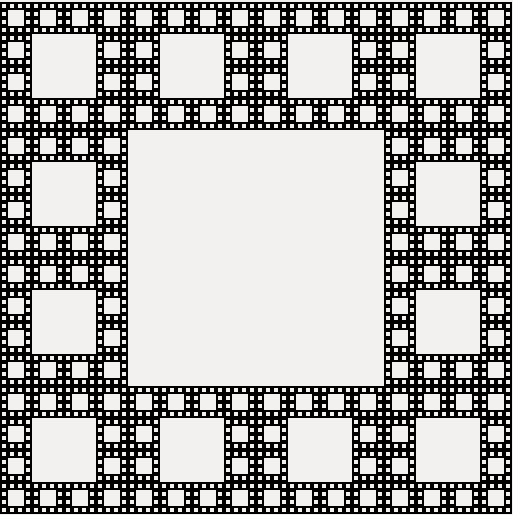
\includegraphics[scale=0.5]{carpet.jpg}
\end{center}

Prenons une macro-cellule de taille n, nous pouvons alors la découper
en 8 macro-cellules de taille égale n-2. Dans les quatre
macro-cellules de taille n-2 au centre, nous y mettons du vide, et
dans toutes les autres on appelle récursivement cette construction
jusqu'à avoir une macro-cellule de taille 1 ou 0, dans ce cas nous
aurons des cellules vivantes. Par conséquent, dans notre cas, nous ne
pouvons avoir que des tapis de Sierpinski de taille n, soit une grille
de 2\textsuperscript{n}x2\textsuperscript{n} avec n pair.

L'intérêt d'une telle fractale est le niveau de redondance de la
structure, on peut facilement imaginer que ce tapis ne prendra que
très peu de place en mémoire malgré une très grande taille. En effet,
cela se confirme : pour un tapis de taille 6 nous
obtenons la représentation en mémoire suivante :

\begin{center}
  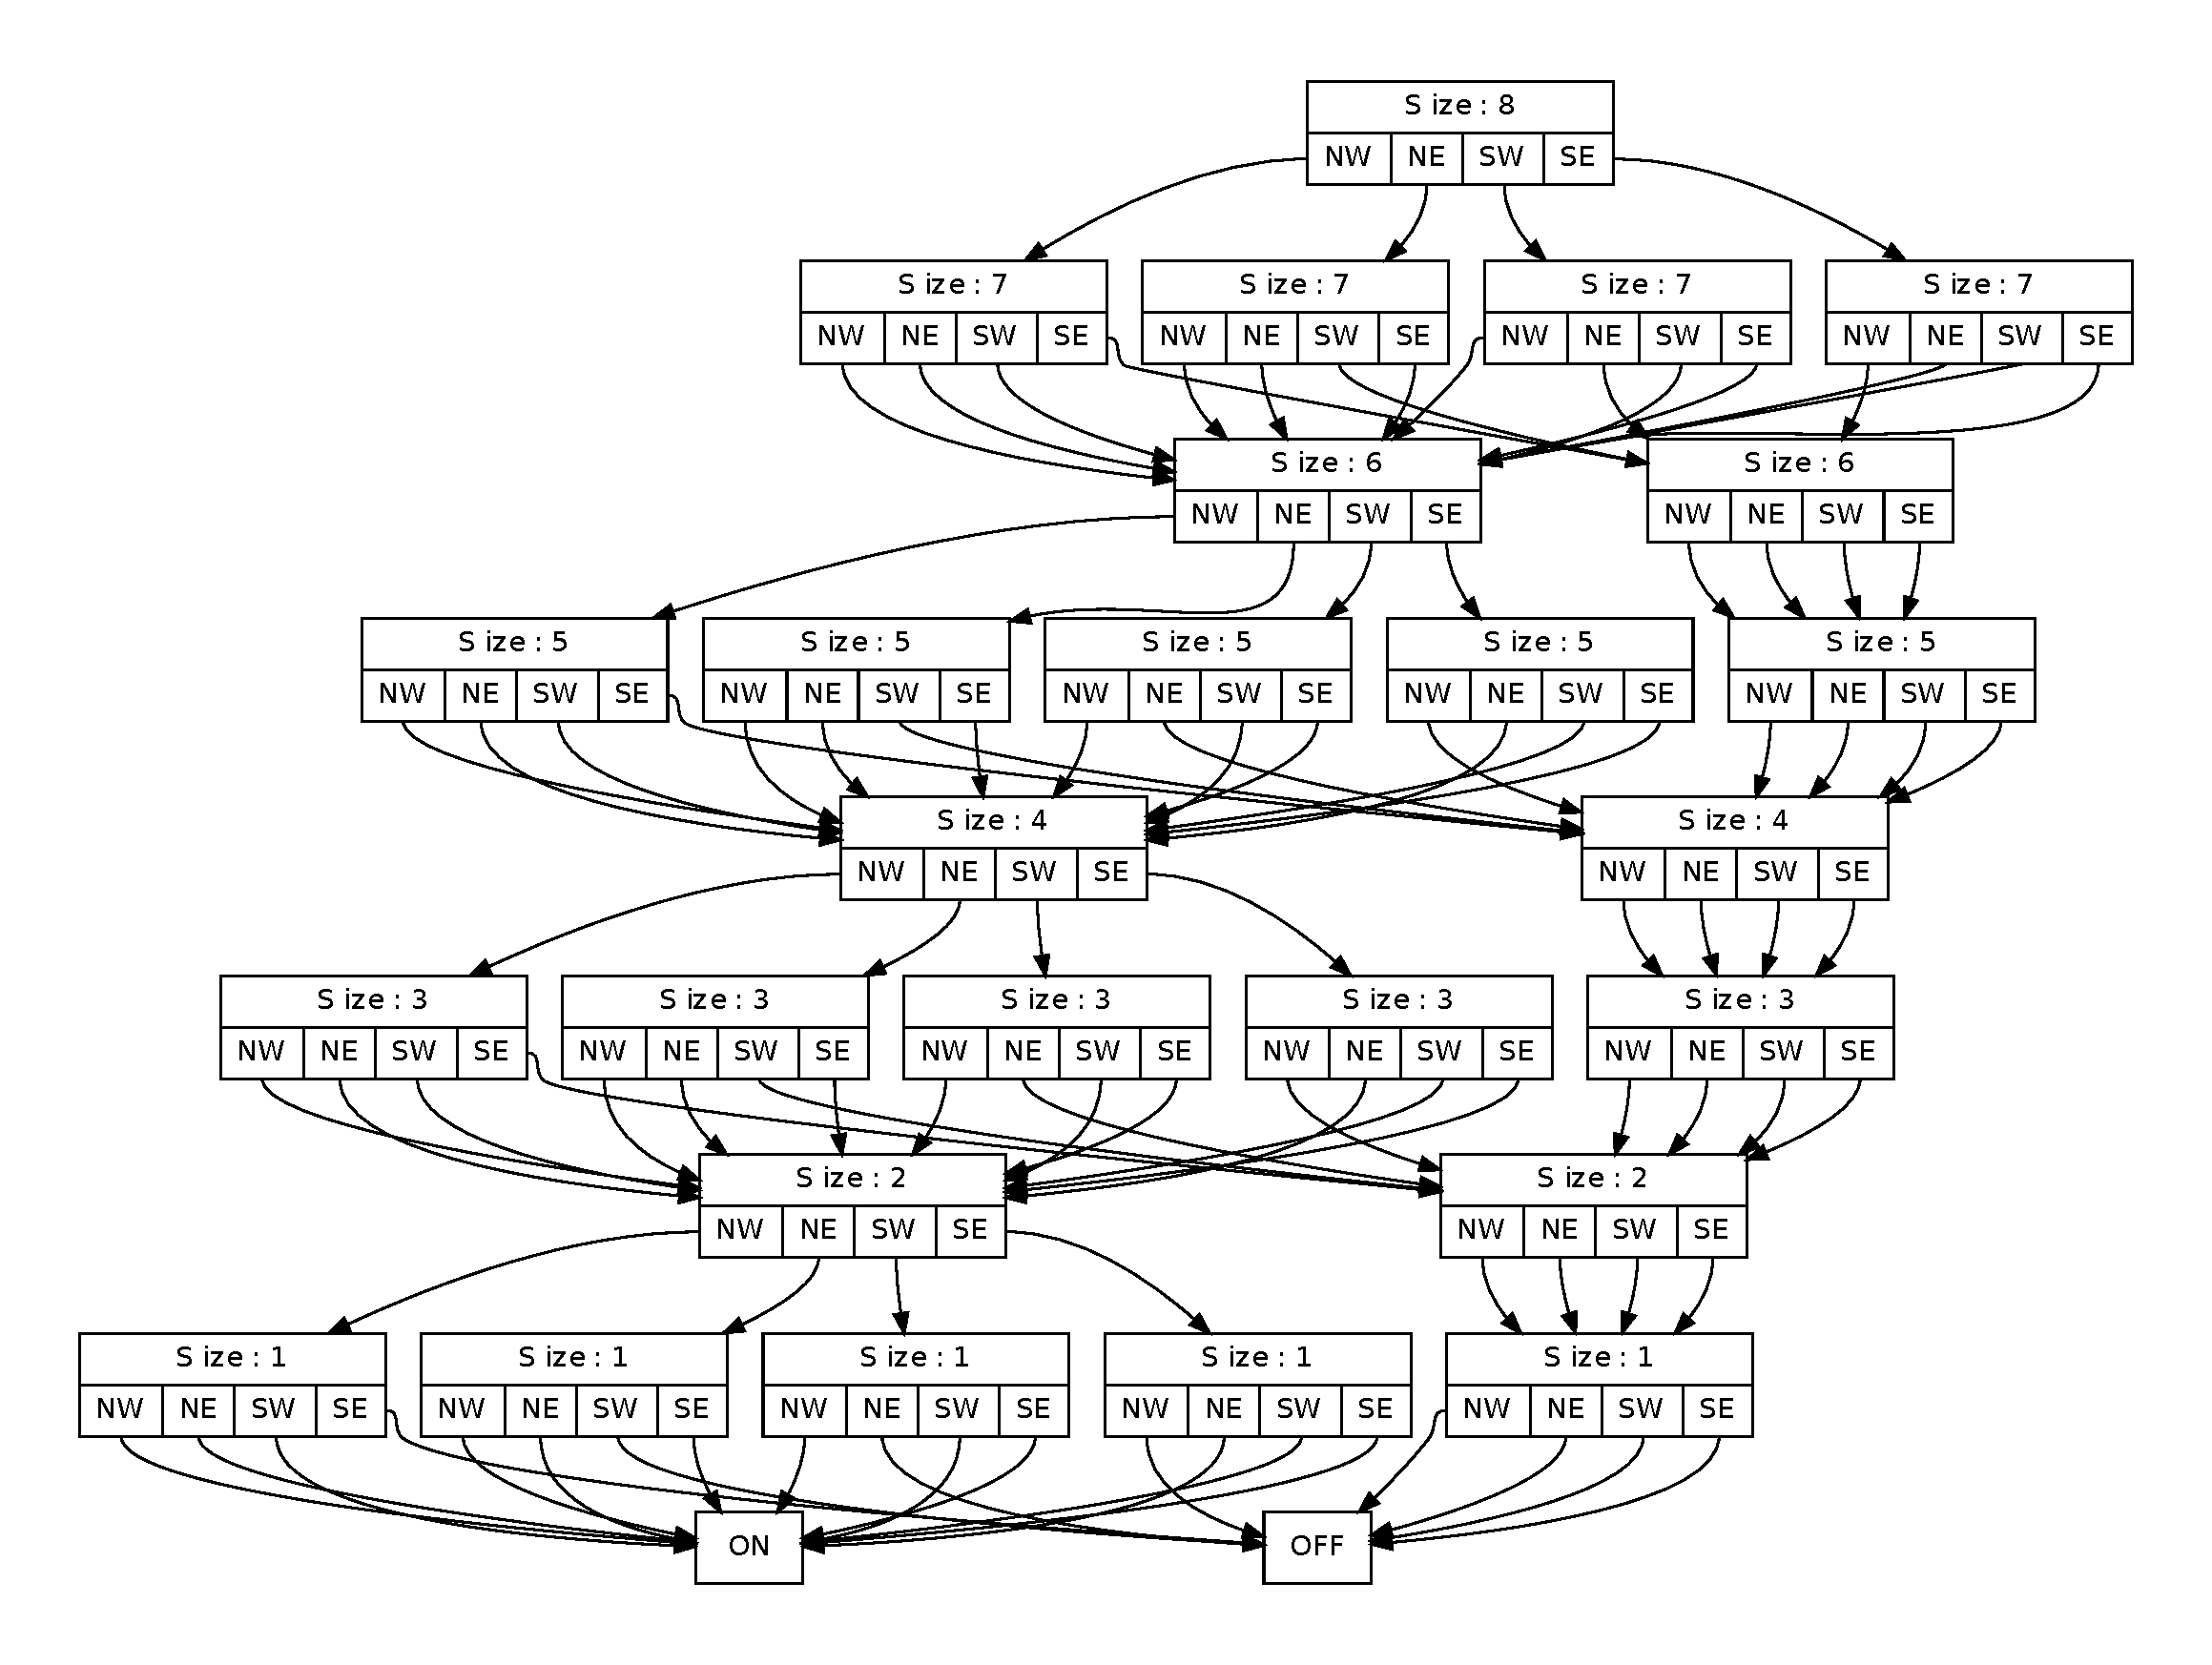
\includegraphics[scale=0.40]{memCarpet6.pdf}
\end{center}

Nous allons donc effectuer les tests suivants, selon la taille n du
tapis : le calcul du nombre de n\oe uds en mémoire du tapis (comme
ci-dessus pour n=6), la mesure du temps de calcul du résultat, ainsi
que le nombre de cellules créés pour le calcul du résultat du tapis.

Étant donnée la structure de la fractale, nous nous attendons à avoir
des résultats linéaires en fonction de n.

\begin{center}
  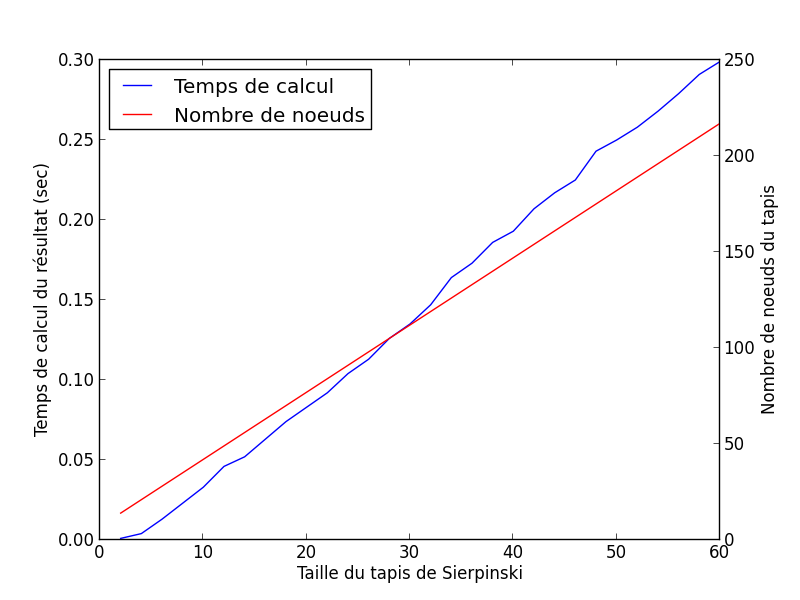
\includegraphics[scale=0.65]{carpet_time_cnt.png}
\end{center}
\begin{center}
  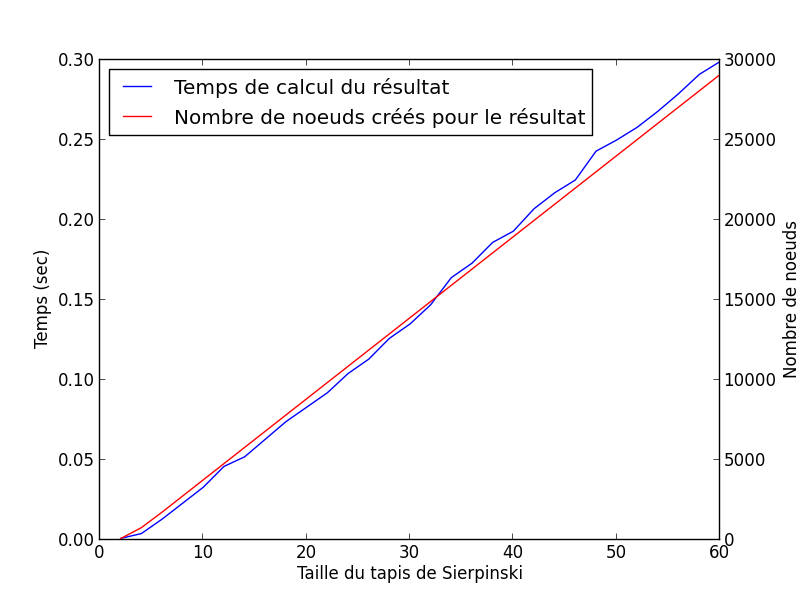
\includegraphics[scale=0.65]{carpet_time_created.png}
\end{center}

Nous observons bien un temps de calcul du résultat linéaire par
rapport à n, tout comme le nombre de n\oe uds créés pour le résultat et
le nombre de n\oe ud du tapis aussi, malgré une taille qui augmente de
façon exponentielle.

Avec cette configuration du tapis de Sierpinski, pour une taille n,
nous avons un total de 12\textsuperscript{ n/2 + 1} cellules
vivantes. À titre indicatif, pour n=42, donc une macro-cellules de
2\textsuperscript{42}, nous avons un total de 5.52e+23 cellules
vivantes, et le calcul du résultat (état de la macro-cellule dans
2\textsuperscript{40} pas de temps) se fait en 207ms en créant
seulement 19 971 macro-cellules intermédiaires pour ce calcul.

\section{Tests sur le glider sur l'espace}

Intéressons-nous maintenant à une configuration qui s'évade dans
l'espace, c'est-à-dire qui va se déplacer à l'infini dans une
direction : l'exemple le plus simple est le glider, qui retourne à son
état d'origine toutes les quatre itérations mais avec une translation
d'une case vers la droite et le bas (variable selon l'orientation du
glider).

\medskip

\begin{center}
  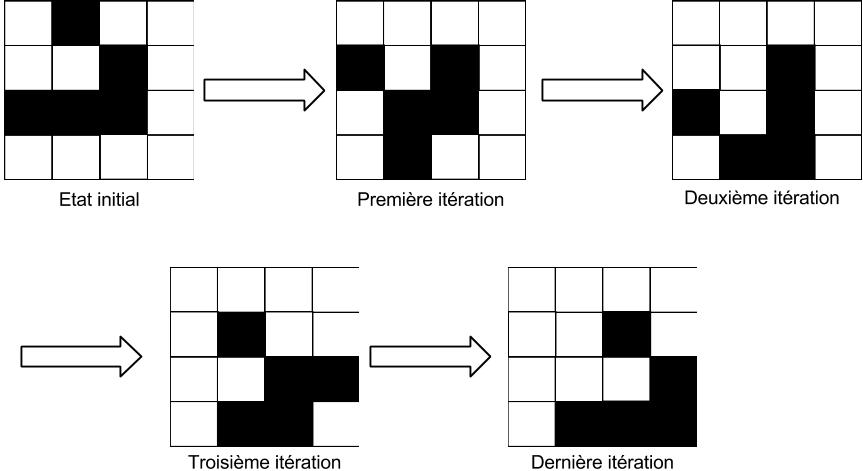
\includegraphics[scale=0.4]{glider_iterations.png}  

  \textit{Les différentes itérations du glider}
\end{center}

\medskip


L'intérêt de l'étude d'une telle configuration est le suivant : le
motif est toujours le même à un pas de temps de 4, mais au fur et à
mesure de ses déplacements, le découpage fait par l'algorithme
Hashlife ne sera pas le même, on observera donc son comportement
notamment au niveau de la création de nouvelles macro-cellules. De
plus, plus le glider avance, plus notre macro-cellule va devoir
s'agrandir.

Nous allons donc lancer un glider et calculer son \texttt{future} dans n pas de
temps en faisant varier n. À noter que les tests sont indépendants les
uns des autres. Nous allons relever : la taille de la macro-cellule
après le calcul du future, le temps de ce calcul, et le nombre de
n\oe uds créés lors de ce calcul.

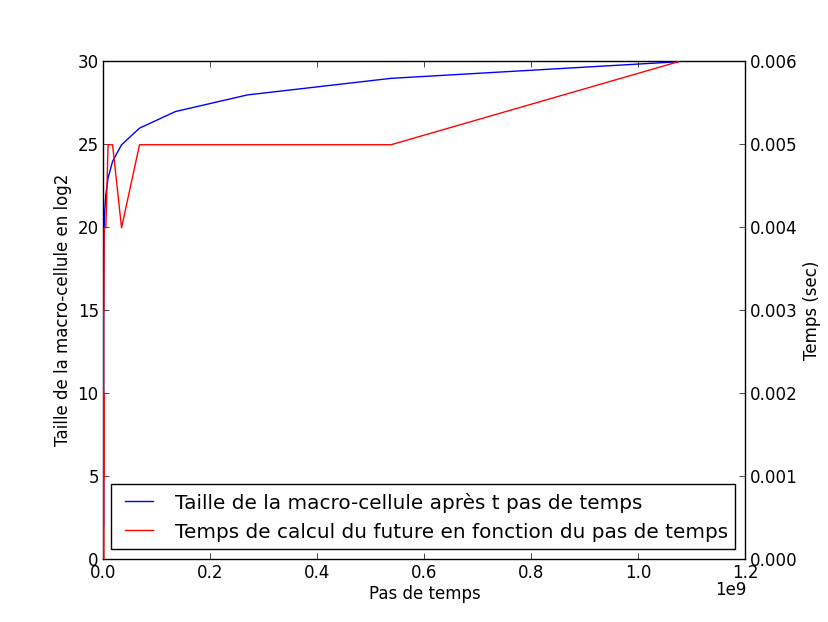
\includegraphics[scale=0.7]{glider_future.png}

Nous pouvons observer que malgré l'augmentation de la taille de la
macro-cellule, le temps de calcul du \texttt{future} reste constant à
2 millième de seconde près, prouvant ainsi l'efficacité de ne traiter
que les cellules pertinentes selon les règles du jeu de la vie. Et par
conséquent, la taille d'une macro-cellule seule n'est pas
représentatif par rapport au temps de calcul du \texttt{future}, il
faut alors prendre aussi en compte le nombre de cellules vivantes
comme lors de nos tests généraux.

\section{Tests sur le ticker sur le temps}

Et pour finir, nous allons prendre une configuration du jeu de la vie
qui devient cyclique à partir d'un certain point dans le but de voir
l'utilisation de la mémoire de nos macro-cellules. Dans ce cas, étant
donné qu'à partir d'un certain temps la configuration est cyclique, on
retrouvera des macro-cellules déjà créées et utilisées donc la mémoire
devrait augmenter en début d'exécution puis stagner.

Donc pour ce test, nous allons lancer la configuration du ticker, et
avec un certain pas de temps, mesurer la taille de la table de
hachage où sont enregistrées les macro-cellules au cours des
itérations successives.

\medskip

Nous obtenons les résultats suivants :

\begin{center}
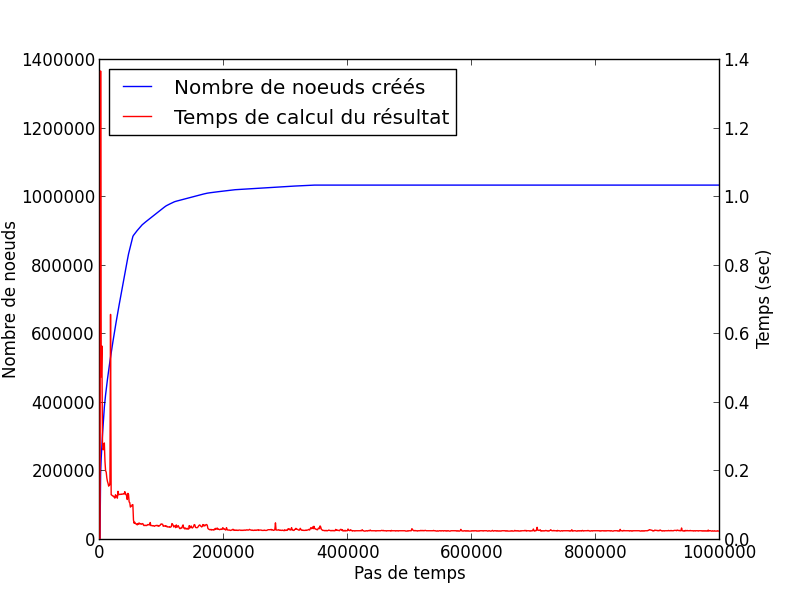
\includegraphics[scale=0.75]{ticker.png}
\end{center}

Comme attendu, nous pouvons constater une augmentation significative
de la mémoire en début d'exécution et à partir de la 6000ème
itération, la mémoire est stable et n'augmente plus. Donc nous pouvons
faire les calculs du résultat de cette configuration instantanément
malgré sa taille de 11 et sur des pas de temps aussi grands qu'on le
souhaite, ce qui démontre l'efficacité de l'algorithme Hashlife et du
hash-consing sur des configurations cycliques au cours du temps.





\chapter{Utilité de ce TER}

\section{Techniques et algorithmique}

Il va de soit que le jeu de la vie a des utilités très limitées en
dehors de l'automate lui-même, mais
ce n'est pas le cas des algorithmes et des techniques qu'on a
utilisés. En effet, plusieurs techniques peuvent être réutilisées
dans d'autres circonstances.

En premier lieu, la mémoïsation et le hash-consing
peuvent être mis en \oe uvre dans de nombreux contextes.
En particulier, la mémoïsation est une alternative élégante à la
programmation dynamique.

De plus, nous avons appliqué dans notre cas, le hash-consing sur des
structures arborescente, que nous pouvons retrouver dans de multiples
problèmes. L'un des cas les plus intéressants est celui des BDD (Binary
Decision Diagram).

Au niveau algorithmique graphique, une macro-cellule n'est rien
d'autre qu'un quadtree et par conséquent afficher un quadtree, qui
n'est pas si évident, est très utilisé dans Google Maps ou bien dans
les GPS pour afficher les cartes.

\section{Outils}

En plus des techniques algorithmiques, nous avons aussi appris à manipuler de
nouveaux outils, ainsi que des concepts utiles pour
mieux programmer.

\medskip

Pour OCaml lui-même, nous avons pu apprendre des concepts un peu plus
avancés et manipuler certaines fonctionnalités telles que les objets
et les arguments labelisés. 

Pendant le développement de notre application, nous avons aussi
utilisé des bibliothèques graphiques en OCaml, mais étant donné que
celles-ci sont essentiellement des bindings des bibliothèques C de Gtk
et Cairo, en apprenant à les utiliser en OCaml, nous avons désormais
une connaissance de ces dernières dans n'importe quel langage, et
ainsi la possibilité de créer des applications graphiques sérieuses
assez rapidement.

Et pour finir, nous avons aussi découvert deux autres outils très
utiles que nous utilisons maintenant très souvent : LaTeX pour rédiger
nos rapports, et SVN/Git pour versionner et travailler en
collaboration.


\medskip

\chapter{Conclusion}

Dans ce TER, nous avons implémenté Hashlife, un algorithme qui permet
de simuler le jeu de la vie à grande échelle de temps et d'espace.

\medskip

Pour cela, il nous a fallu mettre en \oe uvre un mécanisme de
mémoïsation particulier, le hash-consing, nous permettant alors de
sauvegarder des constructions d'arbres et les calculs de résultats. Au
final, il devient alors très facile de représenter des automates du
jeu de la vie dans ce que nous appelons des macro-cellules, autrement
dit des graphes contenant exactement quatre macro-cellules dites
filles. Cette construction permet alors de mettre en avant des
structures redondantes et, assez trivialement, de gagner un facteur
mémoire parfois très important pour des structures présentant
énormément de redondance par rapport à une implémentation naïve du jeu
de la vie (qui serait alors réalisé à l'aide d'une matrice).

\medskip

De la même manière, là où afficher un automate implémenté naïvement
serait relativement facile, il nous fallait écrire un algorithme
capable de dessiner un graphe, et de plus, être capable de dessiner
seulement certaines parties du graphe. Cet algorithme d'affichage de
quadtree peut être d'ailleurs appliqué à d'autres cas différents.

Au delà du jeu de la vie, ce TER nous aura permis de nous familiariser
avec nombre d'outils et de concepts.

\chapter{Remerciements}

Nous remercions principalement Jean-Christophe FILLIÂTRE pour avoir
accepté de superviser notre TER, en nous faisant partager son savoir
et ses méthodes de travail efficaces, et pour tous ces petits moments
culture toujours intéressants.

\medskip

Nous remercions aussi Sylvain CONCHON pour nous avoir mis en relation avec
Jean-Christophe, et dont nous regrettons déjà les enseignements (et ses
déclarations d'amour pour OCaml).

\medskip

Nous remercions l'équipe TOCCATA de nous avoir accueilli dans leurs
locaux, avec le sourire et la bonne humeur.

\medskip

Une attention plus légère mais présente envers nos collègues Rémy
BESOGNET et David DECLERCK pour leur compagnie au sein de
\textit{notre} bureau au LRI et grâce à qui nous avons pu observer une baisse de
productivité (mais on les aime quand même).

\medskip

Merci à Kim NGUYEN (Équipe TOCCATA) pour les dosettes de café, sans
quoi nous n'aurions pas tenu les journées de dur labeur.

\medskip

Enfin, nous souhaitons remercier une fois encore Jean-Christophe et Sylvain,
grâce à qui nous avons pu obtenir un stage chez OCamlPro, et surtout pour nous
avoir transmis leur passion pour OCaml.

\appendix

\chapter{Interface du module MCell}

\input{./ocamldoc.out}


\end{document}

% Local Variables:
% compile-command: "rubber -d rapport.tex"
% ispell-local-dictionary: "francais"
% End:

% LocalWords:  Conway hash-consing Hashlife mémoïsation macro-cellule
% LocalWords:  macro-cellules Implémentation L'implémentation RLE nw
% LocalWords:  sw result Graphics Gtk-Cairo Mcop zoomer implémentable
% LocalWords:  Cairo Gtk widget widgets MC glider.mc mémoïse COUDERC
% LocalWords:  FILLIÂTRE Pierrick David end Mcell Jean-Christophe Rle
% LocalWords:  ticker Golly Gosper mémoïsées mémoïsé mcell foncteur
% LocalWords:  unaires glider Sierpinski turing.rle puffer.rle binôme
% LocalWords:  broken-lines.mc memory-loop.rle hexadecimal.rle rubber
% LocalWords:  hash-consées mémoïsant indentions CONCHON OCamlPro
% LocalWords:  labelisés Decision Diagram Binary LocalWords dosettes
% LocalWords:  compile-command rapport.tex DECLERCK BESOGNET NGUYEN
% LocalWords:  Intéressons-nous
